\documentclass{article}
\usepackage{graphicx}
\usepackage{amsmath}
\graphicspath{ {images/} }
\title{Maths Problems}

\author{Nicholas James}
\begin{document}
\setlength{\parskip}{6pt}
\maketitle{}
\section{A Singular Square}
\subsection{Problem}
\[\overline{AABB}=m^2\]

Find the four digit perfect square where both the first two digits are the same and the last two digits are the same.

\subsection{Solution}

This can be solved in a long winded way by checking whether each of the possible numbers of the form \(\overline{AABB}\) are square. However, I think we would prefer to be a little more clever about it.
Firstly, a good start with problems of this type is to write our number algebraically:

\begin{align*}
  n&=1000A+100A+10B+1B\\
  n&=1100A+11B\\
  n&=11(100A+B)
\end{align*}

So we can see that our number, \(n\), must be divisible by \(11\). Also, as \(n\) is a perfect square, we can also conclude that it must be divisible by \(11^2=121\). Let:

\begin{equation*}
n=m^2
\end{equation*}

As we know that \(n\) is divisible by \(121\) we can see that \(m\) must be divisible by \(11\). At this point we can try all the multiples of \(11\) from \(33\) to \(99\), and we will discover our answer. This has reduced our search size by more than a factor of \(10\). Continuing mathematically, we know,

\begin{equation*}
n=11(100A+B)
\end{equation*}

As \(n\) is divisible by \(121\), we can see that \(100A+B\) is divisible by \(11\). However,

\begin{equation*}
100A+B=99A+(A+B)
\end{equation*}

So, \(A+B\) must be divisible by \(11\). As \(A\) and \(B\) are both less than \(10\), \(A+B=11\). From here we have,

\begin{align*}
  n&=11(99A+11)\\
  \frac{n}{121}&=9A+1
\end{align*}

We know \(n\) is a perfect square, so \(9A+1\) must also be a perfect square. The only possibility is \(A=7 \Rightarrow 9A+1=64\). This gives us,

\begin{equation*}
n=121\times 64=7744=88^2
\end{equation*}

\newpage

\section{Selective Shaking}
\subsection{Problem}

\begin{center}

\includegraphics{handshake}
\end{center}

At a recent party, everyone shook hands exactly once with everyone else. Halfway through the party Magda arrived and shook hands only with the people she likes.

In all there were 201 handshakes.

How many people does Magda like?
\subsection{Solution}
\setlength{\parskip}{6pt}
If everyone in a group of \(n\) people shakes hands with everyone else, there are \( {{n}\choose{2}}= \frac{n(n-1)}{2}\) handshakes.
\renewcommand{\arraystretch}{1.5}
\begin{center}
\begin{tabular}{ |c|c| }

 \hline
 People at party & Handshakes \\
 \hline
 \(19\) & \({{19}\choose{2}}=171\) \\
 \(20\) & \({{20}\choose{2}}=190\) \\
 \(21\) & \({{21}\choose{2}}=210\) \\
 \hline
\end{tabular}
\end{center}

We can see that \(19\) is too few, as Magda would have to shake hands with more people than are present at the party. Similarly, \(21\) is too many, as there would have already been \(210\) handshakes before she arrived.

Therefore, there are \(20\) people at the party, and Magda likes \(201-190=\boxed{11}\) of them.

\newpage

\section{Water into Wine}
\subsection{Problem}
\begin{center}
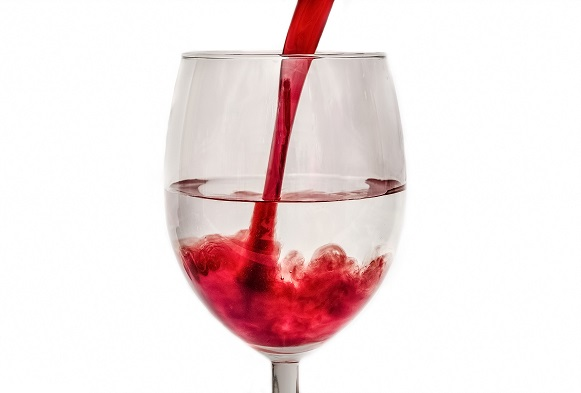
\includegraphics{wine}
\end{center}

One glass contains 100ml of water, and a second glass contains 100ml of wine. 10ml of water is taken from the first glass and put in the second. This mixture is stirred thoroughly, and 10ml is taken and placed back in the first glass.

At the end of this procedure, will the amount of wine in the first glass be greater or smaller than the amount of water in the second glass?

\subsection{Solution}
It is possible to show through a calculation that the amount of water in the second glass is the same as the amount of wine in the first glass. However, there is another way to look at this situation:

At the end of the procedure, the glasses both contain 100ml of liquid. Therefore, any water that is in the second glass must have come from the first glass, and must have been replaced in the first glass by an equal amount of wine.

In fact, the mixing thoroughly step is unnecessary: the result will hold even with substandard mixing practices.

\newpage
\section{Trigonometric Intersections}

\subsection{Problem}

What is the angle between the graphs of \(\tan x\) and \(\cos x\) at their points of intersection?
\subsection{Solution}
\subsubsection{Solution 1}
First, find the points of intersection:

\begin{align*}
\cos(x)&=\tan(x)\\
\cos(x)&=\frac{\sin(x)}{\cos(x)}\\
\cos^2(x)&=\sin(x)\\
1-\sin^2(x)&=\sin(x)
\end{align*}

Solve the quadratic to find:

\begin{equation*}
\sin(x)=\frac{1-\sqrt{5}}{2}
\end{equation*}

Happily, we don't need to find the co-ordinates. Differentiating:

\begin{align*}
d/dx(\cos(x))&=-\sin(x)\\
d/dx(\tan(x))&=-\sec^2(x)
\end{align*}

So, at the intersection, the gradient of \(\cos(x)\) is:

\begin{equation*}
-\sin(x)=-\frac{1-\sqrt{5}}{2}
\end{equation*}

Using the standard labels for a right-angled triangle (O,A,H), we know:
\begin{equation*}
\sin(x)=\frac{1-\sqrt{5}}{2}=\frac{O}{H}
\end{equation*}
\begin{equation}
H(\frac{1-\sqrt{5}}{2})=O
\end{equation}

We know from the problem:
\begin{align*}
  \frac{A}{H}&=\frac{O}{A}\\
  A^2&=OH
\end{align*}

Substitute equation (1):

\begin{align*}
  H^2(\frac{1-\sqrt{5}}{2})&=A^2\\
  \frac{H^2}{A^2}=\sec^2(x)&=\frac{2}{1-\sqrt{5}}
\end{align*}

So, we see that \(\tan(x)\) and \(\cos(x)\) are perpendicular at the intersection points, giving us an answer of \(\pi/2\) for the angle between them.
\subsubsection{Solution 2}
If we know that the tangents are perpendicular, we can prove it in a very succinct way:
\begin{align*}
  f(x)&=\cos(x)\\
  g(x)&=\tan(x)\\
  f'(x)&=-\sin(x)\\
  g'(x)&=\sec^2(x)
\end{align*}

At the points of intersection, \(f(x)=g(x)\)
\begin{align*}
  \cos(x)&=\frac{\sin(x)}{\cos(x)}\\
  1&=\frac{\sin(x)}{\cos^2(x)}
\end{align*}

So we have

\begin{equation*}
  f'(x)g'(x)=-1
\end{equation*}

Which implies the tangents at this point are perpendicular.

\section{Factorial Factors}
\subsection{Problem}
How many numbers are factors of \(21!\) but not of \(20!\)?
\subsection{Solution}
\subsubsection{Solution 1}
A naive approach would suggest that we find the prime decomposition of \(20!\)
\begin{equation*}
  20!=2^{18} \times 3^8 \times 5^4 \times 7^2 \times 11 \times 13 \times 17 \times 19
\end{equation*}
We can see the prime decomposition of \(21!\) will be the same, but with an additional \(3\) and an additional \(7\). We are therefore looking for numbers which have either \(3^9\), \(7^3\) or both as a factor. Our aim is to count the number of factors of \(21!\) that meet these criteria.

For any number we can count its factors by considering its prime composition. Take, for example:

\begin{equation*}
  n=2^x \times 3^y \times 5^z
\end{equation*}

n has \((x+1)(y+1)(z+1)\) factors. This is because there are \(x+1\) posibilities for the number of 2s in each factor (as there can any number from 0 to x of them), and a similar thing is true for 3s and 5s.

Therefore, if we limit the factors of 21! to those which have either \(3^9\), \(7^3\) or both as a factor, we find:
\begin{center}
\begin{tabular}{ |c|c|c|c|c|c|c|c|c|c| }
\hline
Fixed & 2 & 3 & 5 & 7 & 11 & 13 & 17 & 19 & Total \\
\hline
\(3^9\) & 19 & 1 & 5 & 3 & 2 & 2 & 2 & 2 & 4560\\
\(7^3\) & 19 & 9 & 5 & 1 & 2 & 2 & 2 & 2 & 13680\\
\(3^9 \times 7^3\) & 19 & 1 & 5 & 1 & 2 & 2 & 2 & 2 & 1520\\
\hline
\end{tabular}
\end{center}
Totalling these gives us 19760 numbers which are factors of 21! but not 20!.

\subsubsection{Solution 2}
We could also count the number of factors of 21! and subtract the number of factors of 20!. Using the method from solution 1 we find:
\begin{center}
\begin{tabular}{ |c|c|c|c|c|c|c|c|c|c| }
\hline
 & 2 & 3 & 5 & 7 & 11 & 13 & 17 & 19 & Total \\
\hline
\(21!\) & 19 & 10 & 5 & 4 & 2 & 2 & 2 & 2 & 60800\\
\(20!\) & 19 & 9 & 5 & 3 & 2 & 2 & 2 & 2 & 41040\\
\hline
\end{tabular}
\end{center}
Which gives us the same answer of 19760.
\end{document}
